\section{Data}
\label{sec:data}
The dataset used was a mix of the CrowdFlower 
dataset\cite{crowdflower_dataset} and the
Emotions dataset\cite{emotions_dataset}.
The CrowdFlower dataset contains around 40,000 tweets
labeled with 13 different emotions. The Emotions 
dataset contains around 400,000 tweets labeled with 6 
different emotions.

\subsection{Exploratory data analysis and preparation}
Some emotions that are present in the
CrowdFlower dataset were remapped because they
were not present in the Emotions dataset.
The emotions and relative mappings are shown
in \autoref{tab:emotion_mappings}.

\begin{table}[H]
    \centering
    \begin{tabular}{|r|l|}
        \hline
        Emotion & Mapping \\
        \hline
        Happiness & \\
        Sadness & \\
        Anger & \\
        Worry & \\
        Love & \\
        Surprise & \\
        Neutral & \\
        Fun  & Happiness \\
        Relief  & Happiness \\
        Hate  & Anger \\
        Empty  & Neutral \\
        Enthusiasm  & Happiness \\
        Boredom  & Neutral \\
        \hline
    \end{tabular}
    \caption{Emotion mappings, when the mapping is empty the emotion was not remapped.}
    \label{tab:emotion_mappings}
\end{table}

Some instances were removed because they were
duplicates. There were 23,163 duplicates and the
dataset was reduced to 433,646 instances.

\begin{figure}[H]
    \centering
    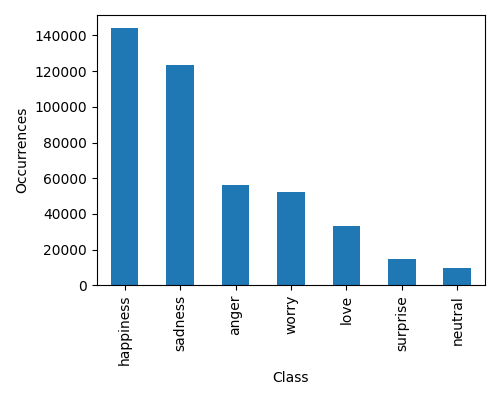
\includegraphics[width=0.48\textwidth]{images/class_distribution.png}
    \caption{Class distribution of the full dataset}
    \label{fig:class_distribution}
\end{figure}

As shown in \autoref{fig:class_distribution},
the dataset is imbalanced. The most common
emotion is Happiness, and the least common
is Neutral. This is because the larger dataset
(Emotions) does not contain the Neutral class.

\begin{figure}[H]
    \centering
    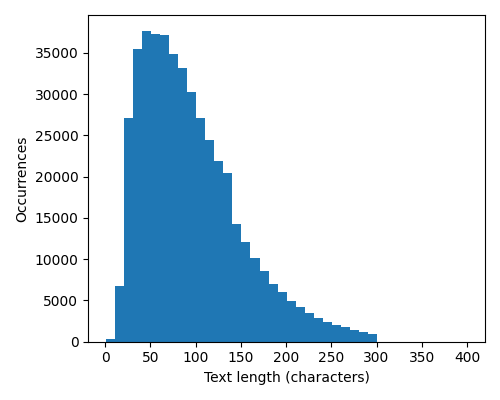
\includegraphics[width=0.48\textwidth]{images/length_distribution.png}
    \caption{Text length distribution of the full dataset}
    \label{fig:length_distribution}
\end{figure}

The dataset was split into a training set
and a test set with a 80\% - 20\% ratio.

\subsection{Preprocessing}
Multiple kinds of preprocessing were tested:
\begin{itemize}
    \item \textit{Bag of words (BoW)}
    \item \textit{Word embeddings (WE)}
    \item \textit{GloVe embeddings (GE)}
\end{itemize}
For the BoW and WE preprocessing, the text was
first cleaned with a regular expression that
removes urls, mentions and symbols. Then the
text was tokenized and stemmed with the 
Snowball stemmer. Both \textbf{TFIDF} and 
\textbf{binary} encodings were tested for
the BoW preprocessing.
The GE preprocessing was done by applying 
the same cleaning regular
expression but without stemming. The vectors
used were the 6B 50d vectors from
GloVe\cite{glove}.
The main difference between the WE and GE
preprocessing is that the WE vectors were
trained on the dataset, while the GE vectors
were pre-trained on a large corpus of text.
